\documentclass[11pt]{article}
\usepackage[margin=0.92in]{geometry}
\usepackage{amsmath,amssymb,graphicx}
\usepackage[hidelinks]{hyperref}
\setlength{\emergencystretch}{1.5em}
\newcommand{\dif}{\mathrm d}
\newcommand{\ii}{\mathrm i}
\title{Separating thermal drift from heat loss by flow reversal in an uncalibrated harmonic sensor array}
\author{% Single-author details supplied on the separate title page.
}
\date{}
\begin{document}
\maketitle
\begin{abstract}
Heat advection and distributed heat loss both attenuate a temperature wave. If heater strengths and receiver sensitivities are unknown, one-way measurements admit a continuum of indistinguishable velocities and loss rates, even when complex responses are available at multiple frequencies. For two heaters bracketing two receivers, we derive this ambiguity and show how an equal-magnitude flow reversal removes it. A four-channel amplitude ratio at two frequencies identifies effective thermal diffusivity; a second ratio across flow directions isolates drift. The latter identity also holds on a finite interval with fixed-temperature ends. We compare closed-form amplitude inversion with a fit to complex responses that estimates receiver gains and eliminates heater amplitudes analytically. In a finite-difference benchmark with a common absolute noise floor, the two methods recovered all three parameters within 10\% in 16 and 266 of 300 realizations, respectively. Supplying the true relative receiver gains increased the latter count to 275. A 5\% direction-dependent change of relative receiver gain produces a velocity bias that can be indistinguishable from true drift. These results separate the calibration removed by flow reversal from the stability still required of a physical sensor.
\end{abstract}
\noindent\textbf{Keywords:} thermal waves; inverse heat transfer; advection--diffusion; structural identifiability; flow reversal; heat loss

\section{Introduction}
A heater can generate measurable oscillations at a downstream thermometer while producing a barely detectable response upstream. The difference carries information about advection, but the two amplitudes also depend on the thermometers, the heater and heat lost to the surroundings. Consider a laboratory flow cell in which a pump can be reversed and the detectors stay in place. Which transport parameters could be recovered from these measurements even if the instruments were noiseless? Which would remain practically measurable when the weakest channel is near the noise floor?

Thermal probes have long been used to infer heat transport and water flux jointly; geometry and dispersion affect those inversions \cite{hopmans}. Alternately heating the upstream and downstream sides has been proposed in flow transducers \cite{transducer}. Dijkstra et al.\ used harmonic power balancing and lock-in detection in a microchannel sensor to suppress drift \cite{dijkstra}. In a different geometry, Deng et al.\ developed a transient double-ratio method with one heater and three sensors to estimate sap velocity and diffusivity \cite{deng}. Effective probe spacing can itself require in situ calibration \cite{kinar}. Noise comparisons in heat-pulse sensing show the value of fitting a full response instead of extracting a few summary statistics \cite{noise}.

Here the uncertain quantities are separate complex factors for every heater drive and receiver channel. The experimental control is reversal of the \emph{medium's motion}, with the receiver channels held fixed. We identify a family of indistinguishable one-way records, construct a two-frequency recovery formula, and derive the specific gain drift that aliases into velocity. We then test the value of retaining complex lock-in data at a fixed number of observations. The application throughout is a homogeneous channel with a linear heat leak. The observations are synthetic.

\section{Transport and measurement model}
Let $T$ be temperature relative to a constant ambient reference. Its cross-sectionally averaged balance is
\begin{equation}
 T_t=D T_{xx}-vT_x-\lambda T+q,\qquad D>0,\quad \lambda\ge0. \label{eq:pde}
\end{equation}
Here $D$ is effective longitudinal thermal diffusivity, $v$ the signed thermal transport speed, and $\lambda$ the lumped loss rate. For a uniform channel of area $A_c$, wetted perimeter $P$, volumetric heat capacity $C$ and a constant linear wall conductance per area $h$, a lumped description gives $\lambda=hP/(C A_c)$. The model assumes small temperature excursions, uniform coefficients, and sufficiently rapid transverse equilibration or spatial averaging. It does not identify wall conductance and heat capacity separately. Relating $v$ to a volumetric flow additionally requires a model for the moving and stationary heat capacities.

\begin{figure}[ht]\centering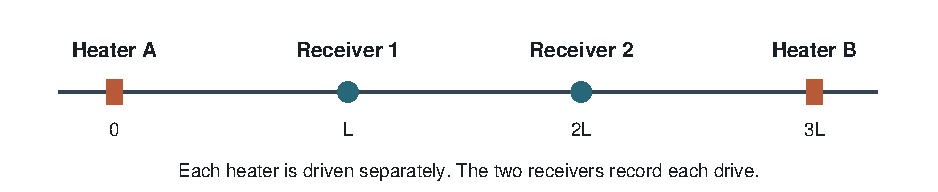
\includegraphics[width=.91\linewidth]{layout.pdf}
\caption{Heater and receiver positions on the transport axis. Both directions of imposed flow use the same four positions. Vector schematic generated by a Python script prepared with OpenAI Codex.}\label{fig:layout}\end{figure}

Use the time convention $e^{\ii\omega t}$ with $\omega>0$. The point-heater response on the infinite line at signed distance $d$ is
\begin{equation}
 G_v(d,\omega)=\frac{\exp(\beta d/2-\kappa |d|)}{2D\kappa},
 \quad \beta=v/D,\quad \kappa^2=\beta^2/4+(\lambda+\ii\omega)/D,\quad
 \operatorname{Re}\kappa>0 . \label{eq:green}
\end{equation}
The substitution $T=e^{\beta x/2}u$ removes the first spatial derivative; continuity and the unit source jump $-D[G']=1$ fix the prefactor. The heaters in Fig.~\ref{fig:layout} are at $z_A=0,z_B=3L$, and the receivers at $x_1=L,x_2=2L$. For flow sign $s=\pm1$ the noiseless response is
\[
 M_{ij}^{s}=g_i(\omega)\,h_j^s(\omega)\,G_{sv}(x_i-z_j,\omega).
\]
The nonzero complex factors allow arbitrary power and phase for each drive, and receiver-specific sensitivity and lag. The relative receiver response $g_2/g_1$ must be the same between the two flow directions at a given frequency. A common receiver gain change can be absorbed into $h_j^s$. Additive cross-talk and flow-dependent probe contact cannot generally be absorbed this way.

\section{Identifiability and its failure modes}
\paragraph{One-way ambiguity.}
Write $B=\beta^2/4+\lambda/D$. Holding $D$ and $B$ fixed preserves $\kappa$ at every frequency. Choose any other $\beta'$ with $\lambda'=D(B-\beta'^2/4)\ge0$. The change in the one-way Green function at $x_i-z_j$ is exactly the product of $e^{(\beta'-\beta)x_i/2}$ and $e^{-(\beta'-\beta)z_j/2}$. Redefining the unknown instrument factors by the reciprocals reproduces all original complex measurements. More frequencies cannot distinguish members of this family under the stated gain model. This result concerns an uncalibrated experiment; an independent known velocity, loss rate or gain ratio supplies different information.

\paragraph{Two-frequency amplitude recovery.}
At either flow direction the cross-ratio satisfies
\begin{equation}
 C^s=\frac{M^s_{1A}M^s_{2B}}{M^s_{1B}M^s_{2A}}=e^{2L\kappa}.
 \label{eq:cross}
\end{equation}
Each instrument factor cancels. The sums of the signed path lengths are equal, while the two short paths total $2L$ and the two long ones $4L$. Write $a_f=\log|C(\omega_f)|/(2L)$. With $\kappa=a+\ii b$, $2ab=\omega/D$ and $a^2-b^2=B$. Therefore, for $0<\omega_1<\omega_2$,
\begin{equation}
 D=\frac12\sqrt{\frac{\omega_2^2/a_2^2-\omega_1^2/a_1^2}{a_2^2-a_1^2}},
 \qquad B=a_1^2-\frac{\omega_1^2}{4D^2a_1^2}.
 \label{eq:d}
\end{equation}
Indeed $a^2=(B+\sqrt{B^2+\omega^2/D^2})/2$ is strictly increasing. Distinct frequencies identify $D$ without unwrapping a phase. Closely spaced frequencies reduce the denominator in Eq.~(\ref{eq:d}). If the phase branch is known independently, a single complex cross-ratio also gives $D=\omega/(2ab)$.

\paragraph{Reversing the flow.}
For either heater and either frequency form
\begin{equation}
 R_j=\frac{M^+_{2j}/M^+_{1j}}{M^-_{2j}/M^-_{1j}}=e^{\beta L},
 \qquad v=D\frac{\log|R_j|}{L},\qquad
 \lambda=D(B-\beta^2/4).
 \label{eq:reversal}
\end{equation}
The heater drops out of each within-drive ratio. Equal-magnitude reversal leaves all the $|d|$ terms invariant. Equation~(\ref{eq:reversal}) identifies the signed speed, including its zero limit. For noiseless measurements $\arg R_j=0$ modulo $2\pi$, and the four values of $\log|R_j|$ agree. Their disagreement can flag inconsistent records; agreement does not certify that the receivers remained stable.

For example, let the relative receiver magnitude in the positive run be $f$ times its value in the negative run. Every $R_j$ is then multiplied by $f$. With $D$ unchanged the inferred speed shifts by $(D/L)\log f$. The change is fully confounded in this geometry: increasing $\beta$ by $\log(f)/L$, changing $\lambda$ to keep $B$ fixed, and multiplying the common receiver ratio by $\sqrt f$ produces the original two sets of within-source ratios, provided the adjusted loss is admissible. Since every heater drive has an arbitrary strength, its absolute level supplies no further constraint. Reducing random noise does not remove this systematic error.

\paragraph{Which identity survives finite ends?}
For a channel $[l,u]$ with zero excess temperature at both ends and a source at $z$, the exact Green function is
\begin{equation}
 e^{\beta(x-z)/2}\,
 \frac{\sinh[\kappa(\min(x,z)-l)]\,\sinh[\kappa(u-\max(x,z))]}
 {D\kappa\sinh[\kappa(u-l)]}. \label{eq:finite}
\end{equation}
Differentiating on either side of $z$ verifies the source jump and the boundary conditions. The fraction is even in $v$. Thus Eq.~(\ref{eq:reversal}) for $v/D$ survives at any end distance, while Eq.~(\ref{eq:cross}) for $\kappa$ generally requires a boundary correction. A velocity estimate that multiplies a boundary-biased $D$ by an unbiased $\beta$ inherits the diffusivity bias.

\section{Estimation from noisy harmonic responses}
Let $y_1,y_2$ be the two complex readings of one heater drive. We compare three estimators on the same sixteen readings (two heaters, receivers, frequencies and directions). The amplitude estimator averages $\log |C^s|$ over directions at each frequency and $\log|R_j|$ over heaters and frequencies, then applies Eqs.~(\ref{eq:d})--(\ref{eq:reversal}). An imaginary diffusivity, a nonfinite estimate, or negative loss is counted as a failure.

For a complex fit, define $\eta_A=-1,\eta_B=+1$ and the predicted within-drive ratio
\[
 Q_{sfj}=\rho_f\exp\{s\beta L/2+\eta_j\kappa_f L\},\qquad \rho_f=g_2(\omega_f)/g_1(\omega_f).
\]
The two noiseless readings lie on the complex line $(t,tQ_{sfj})$ for an unknown $t$ per drive. Minimizing the squared distance to that line over $t$ yields
\begin{equation}
 J=\sum_{s,f,j}\frac{|y_2-Q_{sfj}y_1|^2}{1+|Q_{sfj}|^2}. \label{eq:profile}
\end{equation}
This objective preserves phase without dividing by a noisy observation. It is the profiled negative log likelihood up to constants for independent, equal-variance, circular complex Gaussian errors. Our unknown-gain fit minimizes $J$ over $\log D,\beta,\log\lambda$ and the log magnitudes and phases of two receiver ratios. A calibrated reference supplies the two true receiver ratios while fitting the transport parameters; heater responses remain unknown in all methods. Thus the reference quantifies the benefit of knowing the relative calibration under this design. The two fitted methods impose positive diffusivity and loss; the latter parameterization approaches zero as a limit. The amplitude method is unconstrained, so comparisons include both phase use and differences in estimation and constraints.

A damped Gauss--Newton iteration uses numerical derivatives and starts at $D=0.22$, $\beta=0$, $\lambda=0.045$, $\rho_f=1$ in the unknown-gain case. Units are mm and s. At the baseline noise level, two alternative starts, including one with negative drift, changed fitted parameters by less than $2\times10^{-7}$ relative in all 300 trials. This is a numerical check for that ensemble rather than a global uniqueness result for noisy complex fits. The scripts specify damping, iteration limit and parameter bounds.

\section{Numerical design and verification}
The forward calculation uses a finite channel and centered spatial differences with a nodal point heat source normalized by the grid spacing. The inverse models use the infinite-domain transfer functions. For the baseline set $D=0.15$ mm$^2$/s, $v=0.10$ mm/s, $\lambda=0.03$ s$^{-1}$, $L=2$ mm and $(\omega_1,\omega_2)=(0.025,0.12)$ rad/s. End margins are 20 mm outside each heater. Receiver gains are $1.30/(1+3\ii\omega)$ and $0.72/(1+9\ii\omega)$; heater factors $(0.7,1.4)$ change to $(1.1,0.8)$ on reversal. These are prescribed model parameters, not measured properties of a device.

We compared every raw complex Green response against Eq.~(\ref{eq:finite}) at both frequencies and at $v=-0.10,0,+0.10$ mm/s. Maximum relative complex errors at grid spacings $0.10$, $0.05$, and $0.025$ mm were $1.8314\times10^{-3}$, $4.5802\times10^{-4}$, and $1.1452\times10^{-4}$, close to the expected factor of four under halving. At the finest spacing the clean amplitude inversion returned $(0.149990,0.099996,0.029998)$. At a fixed spacing of $0.05$ mm, reducing the end margin to 2 mm instead gave $(0.15113,0.10076,0.03066)$. These tests verify the implementation within the assumed transport law. They do not validate that law for a fabricated device.

Each complex reading receives independent Gaussian noise of rms magnitude $\sigma$ (variance $\sigma^2/2$ per quadrature). The default absolute floor is $0.01$ times the largest noiseless baseline amplitude. It stays fixed when spacing, frequencies or transport parameters change. The quiet case uses one fifth of this floor. A run succeeds when \emph{all three} errors are below 10\% of their true magnitudes. Nonphysical amplitude solutions remain in the denominator. Trials are independent within each setting; common noise draws align the methods and settings. Computation assumes equally precise harmonic acquisitions at the stated noise floor. The observation count is fixed; actual integration time, settling time and frequency-dependent instrument noise have not been measured. Code generation, numerical analysis and drafting were assisted by OpenAI Codex. Inputs, seeds and executable algorithms accompany the paper.

\section{Results}
\begin{table}[ht]\centering
\caption{Fraction meeting the joint accuracy criterion, reported as counts out of 300. SNR is the weakest noiseless response magnitude divided by the rms noise. The baseline, spacing and frequency rows share an absolute noise floor.}
\begin{tabular}{lrrrr}
Setting & Min.\ SNR & Amplitude & Complex & Calibrated\\ \hline
Baseline &0.76&16&266&275\\
Quiet &3.82&136&300&300\\
$L=1$ mm &6.87&100&264&274\\
$L=1.5$ mm &2.29&61&272&283\\
$L=3$ mm &0.09&1&127&146\\
$\omega_2=0.06$ rad/s &2.13&26&285&291\\
$\omega_2=0.20$ rad/s &0.24&2&250&263
\end{tabular}\label{tab:main}\end{table}

At baseline the median absolute relative errors in $(D,v,\lambda)$ were $(30.1,21.4,50.4)\%$ among physical amplitude estimates, compared with $(2.8,2.9,3.8)\%$ for the complex fit. Seven of the 300 amplitude estimates were nonphysical or nonfinite. The weakest upstream path contributes a log magnitude to the cross-ratio even when its amplitude is dominated by noise. The profiled objective assigns the residual in the original observation units and can draw transport information from the other heater and direction. Supplying the independently calibrated receiver ratios increased the joint success rate from 88.7\% to 91.7\% in this comparison. Approximate marginal 95\% Wilson intervals for 16/300 and 266/300 are 3.3--8.5\% and 84.6--91.8\%; they describe Monte Carlo sampling, not instrument uncertainty.

Increasing $L$ strengthens the ideal logarithmic contrasts in Eqs.~(\ref{eq:cross}) and (\ref{eq:reversal}), but costs exponential attenuation on the long path. At 3 mm the unknown-gain fit succeeded in only 127 trials. Shortening to 1 mm markedly improves the weakest-channel SNR but reduces propagation contrast; it gives 264 successes, comparable to the baseline. There is no universal SNR cutoff in Table~\ref{tab:main}. The lower upper frequency helps here because the high-frequency response also suffers receiver lag. Frequencies arbitrarily close together would eventually destroy amplitude-based conditioning.

For a separate operating map set $\mathrm{Pe}=vL/D$ and $\Lambda=\lambda L^2/D$. We varied these two numbers independently with $D,L$ fixed. The two dimensionless frequencies $\omega L^2/D$ were 0.667 and 3.20. Figure~\ref{fig:map} uses 200 trials per cell. At $\mathrm{Pe}=0.8,\Lambda=0.4$ the unknown-gain fit reaches 191/200; at $\mathrm{Pe}=3,\Lambda=1.6$ it reaches 37/200. Increasing drift strongly attenuates upstream propagation; increasing loss attenuates both paths. At very small loss a 10\% relative tolerance also corresponds to a small absolute error, which explains why success need not rise as loss decreases. The phase-sensitive estimate outperforms the closed form throughout this finite grid. The map is conditional on the chosen receiver responses and noise floor.
\begin{figure}[ht]\centering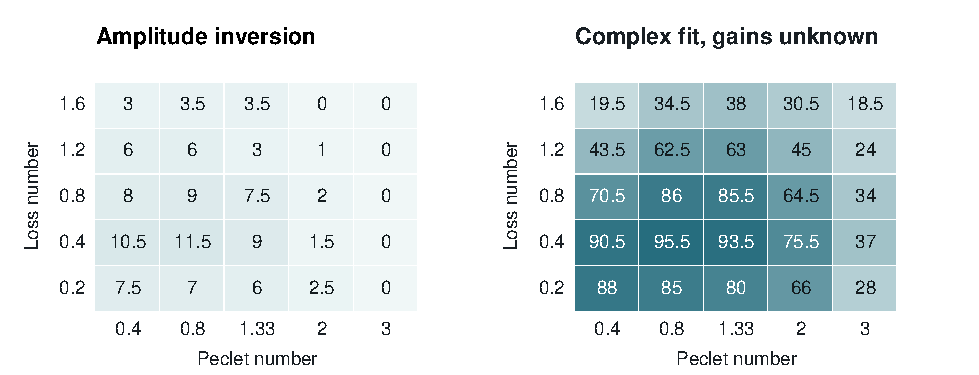
\includegraphics[width=\linewidth]{maps.pdf}
\caption{Percentage of trials recovering $D,v,\lambda$ jointly within 10\%. Both panels use the same finite-domain signals and noise realizations. Each cell represents 200 trials. The numerical data in \emph{regimes.csv} were plotted with a deterministic script prepared with OpenAI Codex.}\label{fig:map}\end{figure}

\paragraph{Departures from the ideal protocol.}
At the quiet noise floor we changed one assumption at a time. Reducing the reverse speed magnitude by 10\% gave a median complex estimate of $v=0.0957$ mm/s. Increasing the positive-run relative receiver gain by 5\% gave $v=0.10368$ mm/s, consistent with the noise-free alias $0.10+(0.15/2)\log(1.05)=0.10366$ mm/s. The latter error cannot be diagnosed from agreement between heaters alone.

To test sensitivity to incomplete transverse equilibration, we added the response of a second axial mode of relative weight 0.35, with effective loss $\lambda+D(\pi/H)^2$, $H=3$ mm. This is the first nonuniform transverse mode of a homogeneous insulated strip with uniform drift. Its weight represents a specified source--receiver coupling; it is a two-mode perturbation rather than a full conjugate wall simulation. The one-mode complex fit returned median $(0.1412,0.0940,0.0309)$ in the adopted units. The downward shifts in diffusivity and speed persist together: the simulated response is a sum of even-in-flow modal envelopes multiplied by the same directional exponential, so the reversal estimate of $v/D$ can remain accurate while the single-mode estimate of $D$ is biased.

\section{Implications for a physical measurement}
Reversal offers two distinct observables. The sign-sensitive reading probes $v/D$ and tolerates fixed-temperature ends. The attenuation and phase contrast probes $D$ and the combined transport loss, and is sensitive to transverse modes, end conditions and insufficient frequency separation. This distinction suggests a direct bench test. Record both complex channels for each heater, use an independent gravimetric or volumetric flow reference in each direction, and measure diffusivity independently in a quiescent sample. A repeat in the original flow direction brackets the reversal in time and tests instrument reproducibility. If the receiver response changes systematically with flow direction, an additional relative-gain reference is necessary. An independent wall cooling measurement would test whether one constant loss coefficient can represent both frequencies.

The conclusions apply to point-like or adequately localized elements, small signals, stable relative receiver transfer functions, and equal-magnitude reversal. Axial wall conduction coupled to the fluid, shear dispersion, unknown source spacing or finite receiver footprints can require an expanded model. Relative-error scores for $v$ and $\lambda$ require nonzero reference values; measurements near zero need absolute error criteria. No experimental data enter the reported comparisons. Their contribution is a testable identifiability result, a finite-boundary benchmark and a quantified example of when a mathematically sufficient amplitude protocol discards practically useful information.

\paragraph{Data and code availability.} The accompanying numerical supplement contains model parameters, finite-difference and inversion code, validation scripts, plotting inputs, and machine-readable result tables. All observations in this study are generated from the stated forward models.
\paragraph{Declaration of generative AI and AI-assisted technologies.} OpenAI Codex was used to develop the identifiability analysis, implement and run the numerical experiments, generate plotting scripts, and draft the manuscript and supplementary materials.

\begin{thebibliography}{9}
\bibitem{hopmans} J.W. Hopmans, J. \v{S}im\r{u}nek, K.L. Bristow, Indirect estimation of soil thermal properties and water flux using heat pulse probe measurements: geometry and dispersion effects, Water Resour. Res. 38 (2002). \href{https://doi.org/10.1029/2000WR000071}{doi:10.1029/2000WR000071}.
\bibitem{transducer} Flow transducer and method, international patent publication WO2004040244A1 (2004). \href{https://patents.google.com/patent/WO2004040244A1/en}{Patent record}.
\bibitem{dijkstra} M. Dijkstra et al., Thermal-wave balancing flow sensor with low-drift power feedback, J. Micromech. Microeng. 24 (2014) 055016. \href{https://doi.org/10.1088/0960-1317/24/5/055016}{doi:10.1088/0960-1317/24/5/055016}.
\bibitem{deng} Z. Deng, H.K. Vice, M.E. Gilbert, M.A. Adams, T.N. Buckley, A double-ratio method to measure fast, slow and reverse sap flows, Tree Physiol. 41 (2021) 2438--2453. \href{https://doi.org/10.1093/treephys/tpab081}{doi:10.1093/treephys/tpab081}.
\bibitem{kinar} N.J. Kinar, J.W. Pomeroy, B. Si, Signal processing for in situ detection of effective heat pulse probe spacing radius as the basis of a self-calibrating heat pulse probe, Geosci. Instrum. Method. Data Syst. 9 (2020) 293--315. \href{https://doi.org/10.5194/gi-9-293-2020}{doi:10.5194/gi-9-293-2020}.
\bibitem{noise} S. Sogala Balaram, V. Srinivasan, Noise-induced errors in heat pulse-based sap flow measurement methods, Agric. For. Meteorol. 350 (2024) 109988. \href{https://doi.org/10.1016/j.agrformet.2024.109988}{doi:10.1016/j.agrformet.2024.109988}.
\end{thebibliography}
\end{document}

